\documentclass[../main]{subfiles}
\begin{document}

\chapter{DSP 开发基础实验}%
\label{cha:test}

\section{实验要求}%
\label{sec:\arabic{chapter}requirement}

\begin{Exercise}
  独立完成项目编译、链接、调试的全过程。
\end{Exercise}

\begin{Answer}
  已完成。
\end{Answer}

\begin{Exercise}
  记录 dataIO()、processing() 子程序的入口地址,记录 currentBuffer.input和
  currentBuffer.output 所在存储器地址。
\end{Exercise}

\begin{Answer}
  \begin{itemize}
    \item 由 CCS 的 Expression 可知地址。
  \end{itemize}
  见表~\ref{tab:address}。
\end{Answer}

\begin{table}[htbp]
  \centering
  \caption{地址}%
  \label{tab:address}
  \csvautobooktabular[respect percent]{tables/address.csv}
\end{table}

\begin{Exercise}
  记录增益控制处理后,以图形方式显示数据空间 currentBuffer.input 和
  currentBuffer.output 缓冲存储器中的波形。
\end{Exercise}

\begin{Answer}
  \begin{itemize}
    \item 由 \url{code/LAB9/sine.dat} 可知输入。
    \item 由输入和程序~\ref{lst:grep}\footnote{搜索 \url{code/LAB9} 文件夹下所
        有含有 INTIALGAIN 或 currentBuffer.output 的内容, -r 递归搜索,即搜
        索当前文件夹的子文件夹, -n 显示行号。} 可知输出是输入的 -4 倍。
  \end{itemize}
  见图~\ref{fig:io}。
\end{Answer}

\begin{listing}[htbp]
  \centering
\begin{windark}{cmd}
> grep 'INITIALGAIN\|currentBuffer.output' -rn code/LAB9
code/LAB9/header/sine.h:21:#define INITIALGAIN -4
code/LAB9/main.c:28:int gain = INITIALGAIN;
code/LAB9/main.c:75:        currentBuffer.output[size] = currentBuffer.input[size] * gain;	// apply gain to input
\end{windark}
  \caption{搜索}%
  \label{lst:grep}
\end{listing}

\begin{figure}[htbp]
  \centering
  \begin{subfigure}[htbp]{0.45\linewidth}
    \centering
    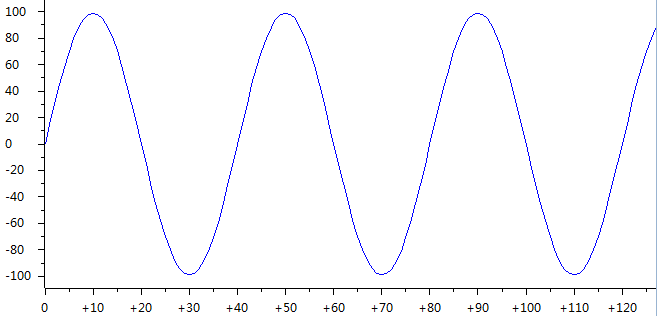
\includegraphics[
      width = \linewidth,
    ]{images/input.png}
    \caption{输入}%
    \label{fig:input}
  \end{subfigure}
  \quad
  \begin{subfigure}[htbp]{0.45\linewidth}
    \centering
    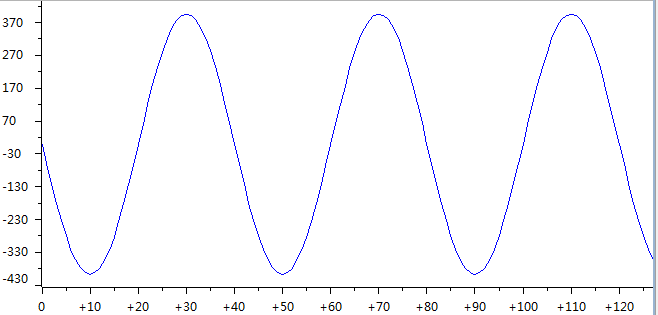
\includegraphics[
      width = \linewidth,
    ]{images/output.png}
    \caption{输出}%
    \label{fig:output}
  \end{subfigure}

  \begin{subfigure}[htbp]{0.45\linewidth}
    \centering
    \begin{tikzpicture}[transform shape]
      \begin{axis}
        \addplot table {data/sine.dat};
        \addplot table {data/gain.dat};
        \legend{currentBuffer.input, currentBuffer.output};
    \end{axis}
  \end{tikzpicture}
  \caption{仿真}%
  \label{fig:io/simulation}
\end{subfigure}
\caption{输入和输出}%
\label{fig:io}
\end{figure}

\begin{Exercise}
  打开工程的 .map 文件,查看所有的段在存储空间的地址和长度,指出分别位于
  TMS320F28335 的什么存储空间以及物理存储块名称。主程序中所用的变量分别属于什
  么段?
\end{Exercise}

\begin{Answer}
  \begin{itemize}
    \item 由 \url{code/LAB9/Debug/LAB9.map} 的 SECTION ALLOCATION MAP 可知段
      的地址和长度。
    \item 由 \url{code/LAB9/Debug/LAB9.map} 的 MEMORY CONFIGURATION 和段的地
      址可知段的存储空间。
    \item 由 \url{https://www.ti.com.cn/cn/lit/gpn/tms320f28335} 156 页的图
      6--23 和段的存储空间可知段的物理存储块名称。
    \item 由 CCS 的 Expression 和段的地址和长度可知变量隶属的段。
  \end{itemize}
  见表~\ref{tab:section}和表~\ref{tab:address}。
\end{Answer}

\begin{table}[htbp]
  \centering
  \caption{段的地址}%
  \label{tab:section}
  \tiny
  \csvautobooktabular[respect all]{tables/section.csv}
\end{table}

\begin{Exercise}
  查看.cmd 命令文件,比较其与上述.map 中的映射关系。试图修改.cmd 文件,再次编
  译链接,查看配置命令与各段的映射关系。
\end{Exercise}

\begin{Answer}
  \url{code/LAB9/28335_RAM_lnk.cmd} 和
  \url{code/LAB9/DSP2833x_Headers_nonBIOS.cmd} 与
  \url{code/LAB9/Debug/LAB9.map} 的映射关系相同。修改
  \url{code/LAB9/28335_RAM_lnk.cmd} 后再次编译链接,
  \url{code/LAB9/Debug/LAB9.map} 和映射关系也会随之变化。
\end{Answer}

\section{实验总结}%
\label{sec:\arabic{chapter}conclusion}

该实验没有难度较大的部分。做完之后我立刻就做下一个了。

一些需要注意的地方:

\begin{itemize}
  \item 如果 CCS 绘图界面始终显示白色,把 CCS 工作目录清空再重新导入工程。这
    是 CCS 5 的漏洞。最迟在 CCS 8 已经修复。
  \item 如果 CCS 绘图的 dual time 不能将 2 个函数画在同一幅图里,而是画在 2
    幅图里,相当于 2 次 single time 。这个设计用处不大。
\end{itemize}

\end{document}
